

 \documentclass[9pt,usenames,dvipsnames]{beamer}%[trans] for handouts
 
 
 \usepackage[T1]{fontenc}
 \usepackage{textcomp}
 \usepackage{ragged2e}
 \usepackage{booktabs}
 \usepackage{fontspec,xltxtra,xunicode}
 \defaultfontfeatures{Mapping=tex-text}
  \setmainfont{Cambria}
 %\setromanfont[Mapping=tex-text]{Hoefler Text}
 %\setsansfont[Scale=MatchLowercase,Mapping=tex-text]{Gill Sans}
 %\setmonofont[Scale=MatchLowercase]{Andale Mono}
  
 \hypersetup{pdfstartview={Fit}}
 
 \title[3-minute thesis 2018]{Yale Linguistics 3-minute thesis 2018}
 \subtitle{Theorising temporomodal interpretation: perspectives from Yolŋu}
 \author{Josh Phillips}
 \institute{Yale Linguistics}
 \date{5 March 2018}
 
  \usepackage{subcaption}
	  \captionsetup{compatibility=false}
% \usepackage{subfigure}
 \usepackage{amsthm}
 \usepackage[normalem]{ulem}
 \usepackage{amssymb}
 \usepackage{multirow}
 \usepackage{mathrsfs}
 \usepackage{pifont}
 \usepackage{mathtools}
 \usepackage{tikz}
 \usepackage{qtree}
 \usepackage{tikz-qtree}
 %\usepackage{tipa}
 \usetikzlibrary{decorations.pathreplacing}
 \usepackage{textcomp}
 \usepackage[normalem]{ulem}
 \usepackage{url}
 \usepackage[all]{xy}
 \usepackage{multicol}
 \usepackage{hanging}
 \usepackage{booktabs}
 \usepackage{setspace}
 \usetikzlibrary{shapes,backgrounds}
 \usepackage{geometry}
 
 
 
% \newtheorem{definition}{Definition}
 %\newtheorem{theorem}{Theorem}
 
 
 \usepackage{enumerate}
 %\usepackage{gb4e} \let\eachwordone=\sl
 \usepackage{expex}
 
 
 
 %\newcommand{\denote}[1]{\mbox{$[\![\mbox{#1}]\!]$}}
 \newcommand{\concat}{\mbox{$^\frown$}}
 \newcommand{\ph}{\varphi}
 \newcommand{\vsep}{\vspace{8pt}}
 \newcommand{\linesep}{\rule{6.5in}{.5pt}}
 \def\attop#1{\leavevmode\vtop{\strut\vskip-\baselineskip\vbox{#1}}}
 \newcommand{\denote}[1]{\mbox{$[\![\mbox{#1}]\!]$}}
 \newcommand{\exref}[1]{~(\ref{#1})}
 
 
 %\input{setup}
 
 %\singlesidestandardsetup
 
 %\parindent 1em
 
 %\input{psfig-scale}
 
 
 \newcommand{\verteq}{\rotatebox{90}{$\,=$}}
 \newcommand{\equalto}[2]{\underset{\scriptstyle\overset{\mkern4mu\verteq}{#2}}{#1}}
 
 
 \newcommand{\secsep}{\hrulefill}
% \renewcommand*{\marginfont}{\small}
 \usepackage{qtree}
 \qtreecenterfalse
 
 \renewcommand{\baselinestretch}{1.2} 
 
 \newcommand{\la}{\langle}
 \newcommand{\ra}{\rangle}
 \newcommand{\lamda}{\lambda}
 \definecolor{ochre}{cmyk}{0, .42, .83, .20}
 \definecolor{forest}{cmyk}{.57, .13, .57, .08}
 \usepackage{framed}
%\usetheme{Warsaw}
%\usecolortheme{wolverine}
	\setbeamercolor{frametitle}{bg=ochre,fg=black}
	\setbeamercolor{title}{bg=ochre,fg=black}
	\setbeamercolor{palette sidebar primary}{use=normal text,fg=normal text.fg}
\iffalse	
	\addtobeamertemplate{navigation symbols}{}{%
		\usebeamerfont{footline}%
		\usebeamercolor[fg]{footline}%
		\hspace{1em}%
		{{\color{ochre!50}\small\textbf{\insertframenumber}}}
	}
\fi
 \begin{document}

\begin{frame}[noframenumbering]{\textbf{Theorising temporomodal interpretation}\hfill\small \textit{perspectives from Yolŋu}}

\pause
\begin{minipage}[l]{0.4\linewidth}
	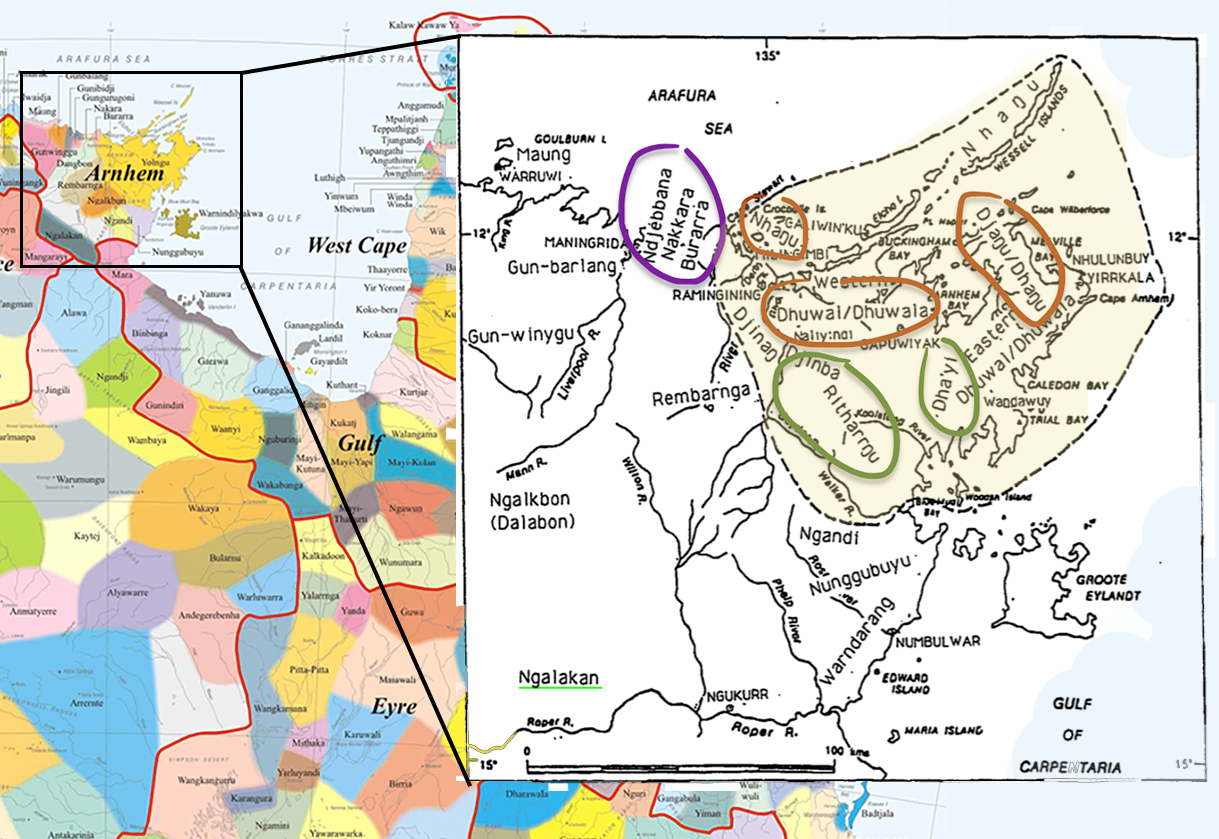
\includegraphics[scale=.11]{AustralianLangsDblCropped}
\end{minipage}
\begin{minipage}[r]{.59\linewidth}
	\begin{itemize}
		\item<3-> Four inflectional categories
		\item<4-> `\textsc{see.}' \textit{\textcolor{Green}{nhäma} -- \textcolor{orange}{nhäŋu} -- \textcolor{blue}{nhäŋal} -- \textcolor{Thistle}{nhänha}}
		\item<5-> Temporal phenomena
		\item<7-> Modal phenomena
		\begin{itemize}\small
			\item<7-> negated propositions
			\item<7-> irrealis (non-realised) predications
			\item<7-> habitual predications
		\end{itemize}
	\end{itemize}
\end{minipage}
\only<5-7>{
\begin{figure}[h]\centering
	\begin{tikzpicture}[scale=.85]
	% draw horizontal line   
	\draw[<->, line width=.5mm] (0,0) -- (12,0);
	
	%draw rex
	\shade[left color=blue!15!white, right color=green!15!white] (0,0.02) rectangle (4.8,1.5);
	%	\fill[green!10!white] (2.5,0.02) rectangle (4.8,1.5);
	\fill[blue!10!white] (4.8,0.02) rectangle (6.8,1.5);
	\fill[green!10!white] (6.8,0.02) rectangle (9.5,1.5);
	\fill[orange!10!white] (9.5,0.02) rectangle (12,1.5);
	
	% draw nodes
	\draw (1.25,0) node[below=3pt] {\textbf{}} node[above=10pt] {\textsc{\textbf{III}}};
	\draw (3.675,0) node[below=3pt] {\textbf{}} node[above=10pt] {\textbf{I}};
	\draw (5,0)   node[circle,fill,label=below:$\lfloor{\sl today}$] {} node[below=3pt] {\textbf{}} node[above=3pt] {};
	\draw (7,0) node[diamond,shade,outer color=black, inner color  = ochre,label=below:$\boldsymbol{t*}$] {} node[below=3pt] {\textbf{}} node[above=3pt] {\textsc{}};
	\draw (5.8,0) node[below=3pt] {\textbf{}} node[above=10pt] {\textsc{\textbf{III}}};	
	\draw (8.15,0) node[below=3pt] {\textbf{}} node[above=10pt] {\textsc{\textbf{I}}};	
	\draw (10.75,0) node[below=3pt] {\textbf{}} node[above=10pt] {\textsc{\textbf{II}}};	
		\draw (9.5,0)   node[circle,fill,label=below:${\sl today}\big)$] {} node[below=3pt] {\textbf{}} node[above=3pt] {};
	
	
	%%%braces
\onslide<6->{
	\draw [decorate,decoration={brace,amplitude=4pt},xshift=-0pt,yshift=35pt]
	(0.5,0.5) -- (4.5,0.5) node [black,midway,yshift=0.35cm] 
	{\footnotesize metricality};}
	\onslide<7->{
	\draw [decorate,decoration={brace,amplitude=4pt},xshift=-0pt,yshift=40pt]
	(3.5,0.5) -- (9,0.5) node [black,midway,yshift=0.35cm] 
	{\footnotesize cyclicity};}
	
	\end{tikzpicture}\end{figure}}


\only<8->{


\begin{figure}[h]	\begin{tikzpicture}[scale=.85]
	% draw horizontal line   
	\draw[<->, line width=.5mm] (0,0) -- (12,0);
	
	%draw rex
	\shade[left color=RoyalPurple!15!white, right color=orange!15!white] (0,0.02) rectangle (4.8,1.5);
	%	\fill[green!10!white] (2.5,0.02) rectangle (4.8,1.5);
	\fill[RoyalPurple!10!white] (4.8,0.02) rectangle (6.8,1.5);
\shade[left color=orange!10!white, right color=Green!10!white] (6.8,0.02) rectangle (9.5,1.5);
	\fill[orange!10!white] (9.5,0.02) rectangle (12,1.5);
	
	% draw nodes
	\draw (1.25,0) node[below=3pt] {\textbf{}} node[above=10pt] {\textsc{\textbf{IV}}};
	\draw (3.675,0) node[below=3pt] {\textbf{}} node[above=10pt] {\textbf{II}};
	\draw (5,0)   node[circle,fill,label=below:$\lfloor{\sl today}$] {} node[below=3pt] {\textbf{}} node[above=3pt] {};
	\draw (7,0) node[diamond,shade,inner color=ochre,outer color=black,label=below:$\boldsymbol{t*}$] {} node[below=3pt] {\textbf{}} node[above=3pt] {\textsc{}};
	\draw (5.8,0) node[below=3pt] {\textbf{}} node[above=10pt] {\textsc{\textbf{IV}}};	
	\draw (7.5,0) node[below=3pt] {\textbf{}} node[above=10pt] {\textsc{\textbf{II}}};
	\draw (9,0) node[below=3pt] {\textbf{}} node[above=10pt] {\textsc{\textbf{I}}};	
	\draw (10.75,0) node[below=3pt] {\textbf{}} node[above=10pt] {\textsc{\textbf{II}}};	
	\draw (9.5,0)   node[circle,fill,label=below:${\sl today}\big)$] {} node[below=3pt] {\textbf{}} node[above=3pt] {};
	
	%braces
	\phantom{	\draw [decorate,decoration={brace,amplitude=4pt},xshift=-0pt,yshift=35pt]
		(0.5,0.5) -- (4.5,0.5) node [black,midway,yshift=0.35cm] 
		{\footnotesize metricality};
		\pause
		\draw [decorate,decoration={brace,amplitude=4pt},xshift=-0pt,yshift=40pt]
		(3.5,0.5) -- (9,0.5) node [black,midway,yshift=0.35cm] 
		{\footnotesize cyclicity};}
	
	\end{tikzpicture}\end{figure}
}
\end{frame}
\end{document}
